\documentclass[letterpaper, 10 pt, journal, twoside]{IEEEtran}
\IEEEoverridecommandlockouts

% Quarto basics minus two problematic packages
\RequirePackage{scrlfile}
\PreventPackageFromLoading{sidenotes}
\PreventPackageFromLoading{marginnotes}


\providecommand{\tightlist}{%
  \setlength{\itemsep}{0pt}\setlength{\parskip}{0pt}}\usepackage{longtable,booktabs,array}
\usepackage{calc} % for calculating minipage widths
% Correct order of tables after \paragraph or \subparagraph
\usepackage{etoolbox}
\makeatletter
\patchcmd\longtable{\par}{\if@noskipsec\mbox{}\fi\par}{}{}
\makeatother
% Allow footnotes in longtable head/foot
\IfFileExists{footnotehyper.sty}{\usepackage{footnotehyper}}{\usepackage{footnote}}
\makesavenoteenv{longtable}
\usepackage{graphicx}
\makeatletter
\def\maxwidth{\ifdim\Gin@nat@width>\linewidth\linewidth\else\Gin@nat@width\fi}
\def\maxheight{\ifdim\Gin@nat@height>\textheight\textheight\else\Gin@nat@height\fi}
\makeatother
% Scale images if necessary, so that they will not overflow the page
% margins by default, and it is still possible to overwrite the defaults
% using explicit options in \includegraphics[width, height, ...]{}
\setkeys{Gin}{width=\maxwidth,height=\maxheight,keepaspectratio}
% Set default figure placement to htbp
\makeatletter
\def\fps@figure{htbp}
\makeatother
\newlength{\cslhangindent}
\setlength{\cslhangindent}{1.5em}
\newlength{\csllabelwidth}
\setlength{\csllabelwidth}{3em}
\newlength{\cslentryspacingunit} % times entry-spacing
\setlength{\cslentryspacingunit}{\parskip}
\newenvironment{CSLReferences}[2] % #1 hanging-ident, #2 entry spacing
 {% don't indent paragraphs
  \setlength{\parindent}{0pt}
  % turn on hanging indent if param 1 is 1
  \ifodd #1
  \let\oldpar\par
  \def\par{\hangindent=\cslhangindent\oldpar}
  \fi
  % set entry spacing
  \setlength{\parskip}{#2\cslentryspacingunit}
 }%
 {}
\usepackage{calc}
\newcommand{\CSLBlock}[1]{#1\hfill\break}
\newcommand{\CSLLeftMargin}[1]{\parbox[t]{\csllabelwidth}{#1}}
\newcommand{\CSLRightInline}[1]{\parbox[t]{\linewidth - \csllabelwidth}{#1}\break}
\newcommand{\CSLIndent}[1]{\hspace{\cslhangindent}#1}

\makeatletter
\makeatother
\makeatletter
\makeatother
\makeatletter
\@ifpackageloaded{caption}{}{\usepackage{caption}}
\AtBeginDocument{%
\ifdefined\contentsname
  \renewcommand*\contentsname{Table of contents}
\else
  \newcommand\contentsname{Table of contents}
\fi
\ifdefined\listfigurename
  \renewcommand*\listfigurename{List of Figures}
\else
  \newcommand\listfigurename{List of Figures}
\fi
\ifdefined\listtablename
  \renewcommand*\listtablename{List of Tables}
\else
  \newcommand\listtablename{List of Tables}
\fi
\ifdefined\figurename
  \renewcommand*\figurename{Figure}
\else
  \newcommand\figurename{Figure}
\fi
\ifdefined\tablename
  \renewcommand*\tablename{Table}
\else
  \newcommand\tablename{Table}
\fi
}
\@ifpackageloaded{float}{}{\usepackage{float}}
\floatstyle{ruled}
\@ifundefined{c@chapter}{\newfloat{codelisting}{h}{lop}}{\newfloat{codelisting}{h}{lop}[chapter]}
\floatname{codelisting}{Listing}
\newcommand*\listoflistings{\listof{codelisting}{List of Listings}}
\makeatother
\makeatletter
\@ifpackageloaded{caption}{}{\usepackage{caption}}
\@ifpackageloaded{subcaption}{}{\usepackage{subcaption}}
\makeatother
\makeatletter
\@ifpackageloaded{tcolorbox}{}{\usepackage[many]{tcolorbox}}
\makeatother
\makeatletter
\@ifundefined{shadecolor}{\definecolor{shadecolor}{rgb}{.97, .97, .97}}
\makeatother
\makeatletter
\makeatother

% Common packages
\usepackage[T1]{fontenc}
\usepackage{lipsum}
\usepackage{amsmath}
\usepackage{amssymb}
\usepackage{physics}
\usepackage{siunitx}
\usepackage{graphicx}
\usepackage[hyphens]{url}
\usepackage{threeparttable}
\usepackage{xcolor}
\usepackage{float}
\usepackage{xcolor}
\usepackage{booktabs}
\usepackage{makecell}
\usepackage{orcidlink}
% monofont
\usepackage[scaled=0.8]{inconsolata}

%styled tabled generated from pandas
\usepackage{colortbl}
\usepackage{multirow}
\usepackage{stfloats} % https://tex.stackexchange.com/a/324358

% Fix table in 2-column format and enable wide table
% https://tex.stackexchange.com/a/224096
\makeatletter
% My tables
\newenvironment{mytable}[1][htbp]{
    \begin{figure}[#1]
    \footnotesize
    \onecolumn
    \begin{minipage}{0.5\textwidth}}
{
    \end{minipage}
    \twocolumn
    \end{figure}}

\newenvironment{mywidetable}[1][tbp]{
    \begin{figure*}[#1]
    \footnotesize
    \onecolumn
    \begin{minipage}{1.0\textwidth}}
{
    \end{minipage}
    \twocolumn
    \end{figure*}}

\renewenvironment{table*}{\begin{mywidetable}}{\end{mywidetable}\ignorespacesafterend}
\renewenvironment{table}{\begin{mytable}}{\end{mytable}\ignorespacesafterend}    
\makeatother



% Muted text (for filler text)
\newcommand\muted[1]{%
\bgroup
\hskip0pt\color{black!40!}%
#1%
\egroup
}

% color links
\usepackage{hyperref}
\hypersetup{ colorlinks, citecolor=teal, linkcolor=teal, urlcolor=teal}


\begin{document}

% author blocks
\author{
        Rainer Koelle\(^1\)\orcidlink{0000-0000-0000-0000},     Second
Author\(^1\)\orcidlink{0000-0000-0000-0000},     Third Author\(^2\)
    \thanks{\(^1\)Performance Review Unit, EUROCONTROL. \(^2\)Some
corporation.}
    \thanks{Released on: }
    \thanks{Extra footnote..}
}


% title
\title{Arrival Management with Open Data}
\maketitle

% abstract
\begin{abstract}
    This document is a sample illustrating the Quarto \texttt{ieeetran}
    template. It includes the key elements of a scientific articles
    (references, equations, figures, tables, code, cross references).
    The template enables the generation of IEEE-formatted article from a
    Jupypter notebook.
\end{abstract}

% body
\hypertarget{introduction}{%
\section{Introduction}\label{introduction}}

Operational efficiency is a key element of addressing aviation's
contribution to climate change. Emissions may increase due to the
expected growth in international air traffic until lower emitting
technologies and fuels and other mitigating measures are developed and
deployed .. ICAO adopted at its 41st Assembly a long-term aspirational
goal for international aviation
\protect\hyperlink{ref-icao2022}{{[}1{]}}. In support to the Paris
Agreement, the goal is to achieve net-zero carbon emissions by 2050.

Levers for fuel reduction:

* operational efficiency

* market-based measures

* sustainable aviation fuel

* new aircraft propulsion and airframes

A wider use and pick-up of sustainable aviation fuel, and new aircraft
propulsion technologies or aircraft design requires further research.

Despite the introduction of an initial market-based mechanism, immediate
action to curb fuel burn and CO2 emissions rests with improvements of
operational efficiency.

The contribution of this paper comprise:

\begin{itemize}
\item
  conceptualisation of sequencing separation for arrival management and
  development of an open data and open software based implementation of
  the approach; and
\item
  use-case application of the developed approach on a subset of airports
  within the European
\end{itemize}

\hypertarget{trajectory-based-operations---arrival-management}{%
\section{Trajectory-Based Operations - Arrival
Management}\label{trajectory-based-operations---arrival-management}}

\hypertarget{header-2}{%
\subsection{header 2}\label{header-2}}

\hypertarget{data-and-conceptual-approach}{%
\section{Data and Conceptual
Approach}\label{data-and-conceptual-approach}}

\hypertarget{approach}{%
\subsection{Approach}\label{approach}}

data preparation

\begin{itemize}
\tightlist
\item
  trajectory data - Opensky Network, weekly downloads
\item
  airport information - Openstreet Map
\end{itemize}

data downloaded \& script development, data cleaning

\hypertarget{trajectory-flight-phase-segmentation-milestone}{%
\subsubsection{Trajectory Flight Phase Segmentation \&
Milestone}\label{trajectory-flight-phase-segmentation-milestone}}

Different approaches exists to detect and describe aircraft flight
phases, e.g.~recent machine learning algorithm
\protect\hyperlink{ref-sun2017flightphase}{{[}2{]}}. This paper
implements a heuristic approach with a focus on the detection of arrival
traffic at the study airports. Figure Figure~\ref{fig-EGLL-arrivals}
shows the detected arrival flights for a single day.

\begin{figure}

{\centering 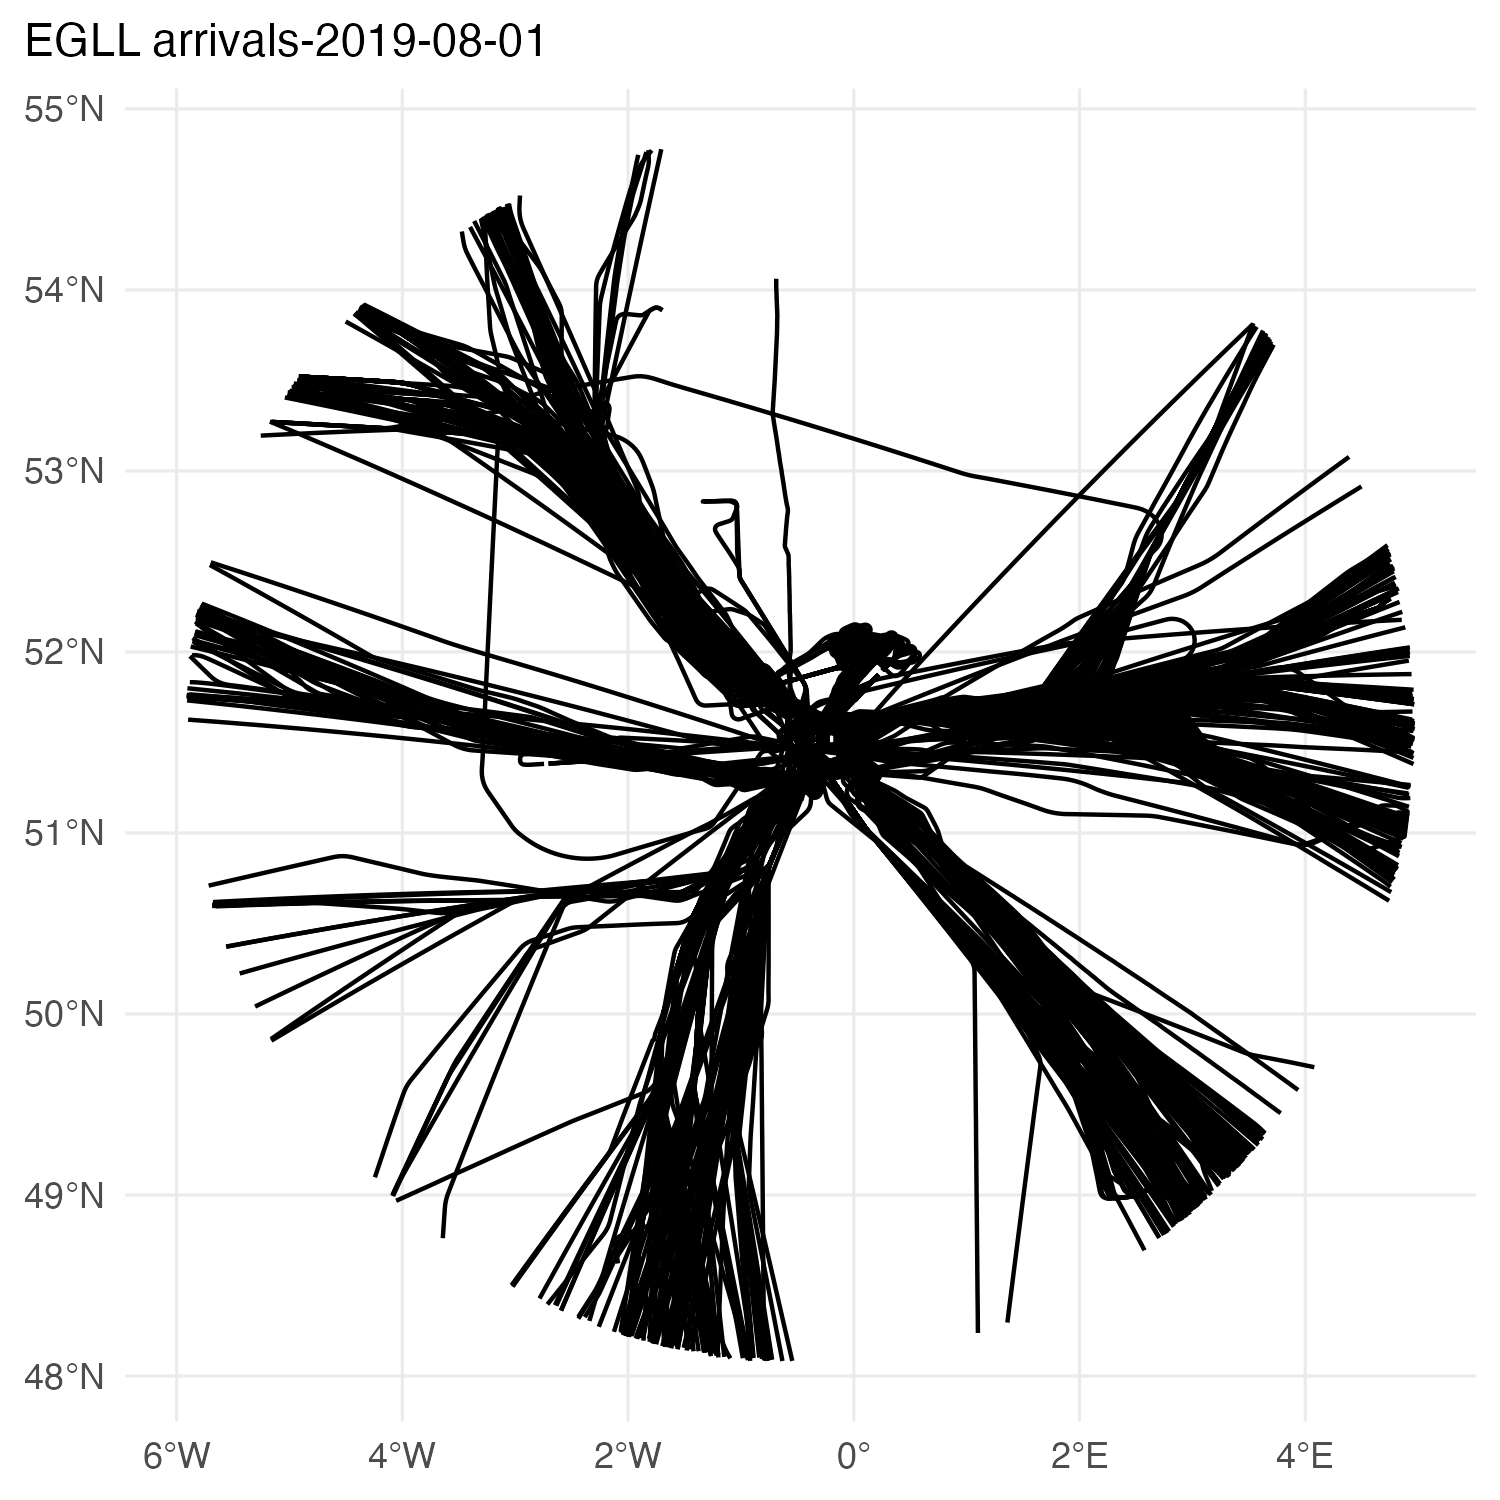
\includegraphics[width=0.45\textwidth,height=\textheight]{./figures/EGLL-arrivals-single-day.png}

}

\caption{\label{fig-EGLL-arrivals}Arrivals at London Heathrow (EGLL) on
sample day}

\end{figure}

\hypertarget{landing-runway-identification}{%
\subsubsection{Landing Runway
Identification}\label{landing-runway-identification}}

The identification of the landing direction is based on a simple
geospatial heuristic. Conceptually, aircraft are aligned with the runway
(centerline) before landing. An aircraft is assigned to a landing runway
based on the closeness of its pre-landing positions to the extended
runway centerline.

\hypertarget{arrival-sequencing}{%
\subsection{Arrival Sequencing}\label{arrival-sequencing}}

Spacing deviation

Let us consider a pair of consecutive landing aircraft denoted leader
and trailer, with s their required time spacing1. Using the constant
time delay principle, the spacing deviation (or spacing error) at time t
considers the current position of trailer at time t, and the past
position of leader at time t -- s. Precisely, it is defined as the
difference between the respective minimum times from these two positions
(see figure below): spacing deviation (t) = min time (trailer (t)) --
min time (leader (t -- s))

\hypertarget{case-study---results}{%
\section{Case Study - Results}\label{case-study---results}}

\hypertarget{data-sampling}{%
\subsection{Data Sampling}\label{data-sampling}}

At the time of writing no global open flight table exists. For this
study, we validated the sample with reference data available to the
Performance Review Unit. Under the EUROCONTROL Performance Review
System, airport operators report movement data on a monthly basis
\protect\hyperlink{ref-apdf_v1_2019}{{[}3{]}}.

\hypertarget{conclusions}{%
\section{Conclusions}\label{conclusions}}

This paper aimed at exploring a data-driven approach to measuring
arrival management based on open data.

\hypertarget{reproducibility}{%
\section*{Reproducibility}\label{reproducibility}}
\addcontentsline{toc}{section}{Reproducibility}

This paper has been built with the R/RStudio ecosystem. The draft
manuscript and its supporting data preparatory steps are archived at
https://github.com/rainer-rq-koelle/paper-2023-ICNS.

The script to download the weekly global datasets are included. The
cleaned trajectory data is stored at:
\textless\textless tbd\textgreater\textgreater.

\hypertarget{acknowledgment-and-disclaimer}{%
\section*{Acknowledgment and
Disclaimer}\label{acknowledgment-and-disclaimer}}
\addcontentsline{toc}{section}{Acknowledgment and Disclaimer}

The authors thank the comments by XX YY ZZ.

The views expressed are the authors' own and do not represent a policy
or position of EUROCONTROL .

\hypertarget{bibliography}{%
\section*{References}\label{bibliography}}
\addcontentsline{toc}{section}{References}

\hypertarget{refs}{}
\begin{CSLReferences}{0}{0}
\leavevmode\vadjust pre{\hypertarget{ref-icao2022}{}}%
\CSLLeftMargin{{[}1{]} }%
\CSLRightInline{ICAO, {``Resolution A41-21: Consolidated statement of
continuing ICAO policies and practices related to environmental
protection {\textemdash} climate change,''} 2022 {[}Online{]}.
Available:
\url{https://www.icao.int/environmental-protection/Documents/Assembly/Resolution_A41-21_Climate_change.pdf}}

\leavevmode\vadjust pre{\hypertarget{ref-sun2017flightphase}{}}%
\CSLLeftMargin{{[}2{]} }%
\CSLRightInline{J. Sun, J. Ellerbroek, and J. Hoekstra, {``Flight
extraction and phase identification for large automatic dependent
surveillance\textendash broadcast datasets,''} \emph{Journal of
Aerospace Information Systems}, vol. 14, no. 10, pp. 566--572, 2017. }

\leavevmode\vadjust pre{\hypertarget{ref-apdf_v1_2019}{}}%
\CSLLeftMargin{{[}3{]} }%
\CSLRightInline{EUROCONTROL, {``Eurocontrol {Specification} for
{Operational ANS Performance Monitoring} - {Airport Operator Data
Flow}.''} 2019 {[}Online{]}. Available:
\url{https://www.eurocontrol.int/publication/eurocontrol-specification-operational-ans-performance-monitoring}}

\end{CSLReferences}

% done
\end{document}
